\documentclass{book}
\usepackage{graphicx}

\title{Test Book}
\author{Author}

\newif\ifplastex
\plastexfalse

\begin{document}

\frontmatter

\ifplastex
    \usepackage{localdef}
    \maketitle

\else

\fi

\chapter{Chapter}

\newcommand{\tbl}[2]{#2\caption{#1}}

Figure~\ref{nsfg_hist} shows histograms of pregnancy lengths for
first babies and others.
\index{pregnancy length}
\index{length!pregnancy}

\begin{figure}
% descriptive.py
\centerline{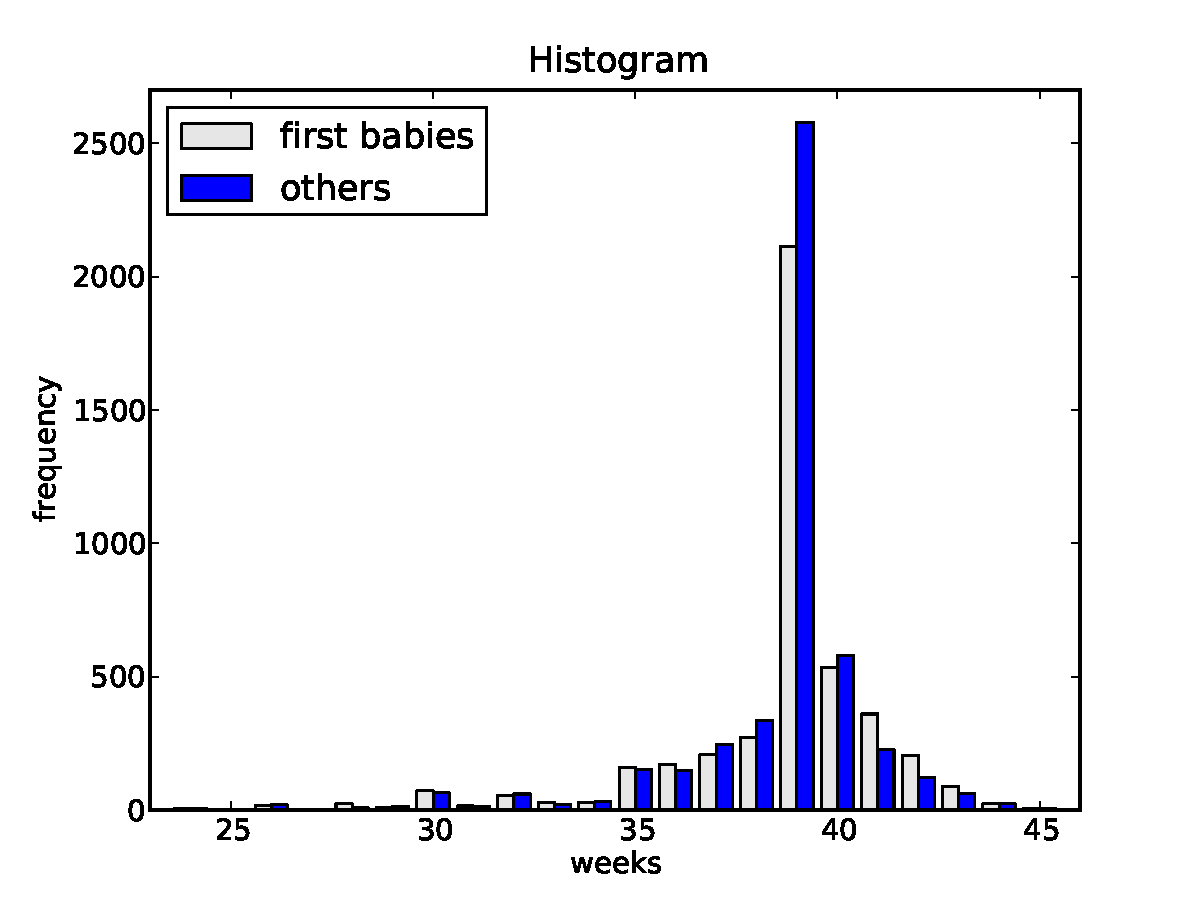
\includegraphics[scale=0.5]{figs/nsfg_hist.pdf}}
\caption{Histogram of pregnancy lengths.}
\label{nsfg_hist}
\end{figure}

\begin{unnumlist}
\subparagraph{Accuracy}
\item \index{accuracy!defined} Accuracy expresses how close the result of a calculation
  or measurement comes to the ``true'' value. Low accuracy is due to
  systematic error.
\subparagraph{Precision} \index{precision!defined} 
\item Precision refers to the ``margin of error'' \index{margin of error} in the 
  calculation or the experiment. In experimental situations, precision
  tells us how far the results will stray when the experiment is 
  repeated several times. Low precision is due to random noise.
\end{unnumlist}


\begin{table}
\tbl{The first 30 job titles and their relative frequencies.\label{tbl:jobtitles}}{%
\begin{tabular}{lrrr}
\toprule
   & \textbf{Number of}
   & \textbf{Fraction of}
  & \textbf{Cumulative} \\
\textbf{Title} &  \textbf{customers} & \textbf{customers} & \textbf{fraction}\\
\colrule
Teacher \rule{0mm}{4mm}  & 66,470  &  0.34047   &   0.340 \\ 
Principal                & 22,958  &  0.11759   &   0.458 \\
Superintendent           & 12,521  &  0.06413   &   0.522 \\
\botrule
\end{tabular}}
\end{table}



\end{document}

